\documentclass[12pt,letterpaper]{article}

\newenvironment{proof}{\noindent{\bf Proof:}}{\qed\bigskip}

\newtheorem{theorem}{Theorem}
\newtheorem{corollary}{Corollary}
\newtheorem{lemma}{Lemma} 
\newtheorem{claim}{Claim}
\newtheorem{fact}{Fact}
\newtheorem{definition}{Definition}
\newtheorem{assumption}{Assumption}
\newtheorem{observation}{Observation}
\newtheorem{example}{Example}
\newcommand{\qed}{\rule{7pt}{7pt}}

\newcommand{\assignment}[4]{
\thispagestyle{plain} 
\newpage
\setcounter{page}{1}
\noindent
\begin{center}
\framebox{ \vbox{ \hbox to 6.28in
{\bf CS412: ntroduction to Data Mining \hfill #1}
\vspace{4mm}
\hbox to 6.28in
{\hspace{2.5in}\large\mbox{Problem Set #2}}
\vspace{4mm}
\hbox to 6.28in
{{\it Handed Out: #3 \hfill Due: #4}}
}}
\end{center}
}

\newcommand{\solution}[4]{
\thispagestyle{plain} 
\newpage
\setcounter{page}{1}
\noindent
\begin{center}
\framebox{ \vbox{ \hbox to 6.28in
{\bf CS412:   Introduction to Data Mining \hfill #4}
\vspace{4mm}
\hbox to 6.28in
{\hspace{2.5in}\large\mbox{#3}}
\vspace{4mm}
\hbox to 6.28in
{#1 \hfill {\it #2}}
}}
\end{center}
\markright{#1}
}

\newenvironment{algorithm}
{\begin{center}
\begin{tabular}{|l|}
\hline
\begin{minipage}{1in}
\begin{tabbing}
\quad\=\qquad\=\qquad\=\qquad\=\qquad\=\qquad\=\qquad\=\kill}
{\end{tabbing}
\end{minipage} \\
\hline
\end{tabular}
\end{center}}

\def\Comment#1{\textsf{\textsl{$\langle\!\langle$#1\/$\rangle\!\rangle$}}}


%\documentclass{article}
\usepackage{amsmath}
\setlength{\parindent}{0pt}
\usepackage{graphicx}
%\usepackage{fullpage}
%\usepackage{setspace} 
\usepackage{float}
%\usepackage{listings} 
%\usepackage{bbm}
\usepackage{bigstrut}
%\usepackage{caption}
%\usepackage{subcaption}
%\usepackage{algpseudocode}
%\usepackage{algorithm}
\usepackage{graphicx}
\graphicspath{ {images/} }

\usepackage{listings}
\usepackage{color}
\usepackage[utf8]{inputenc}

\definecolor{dkgreen}{rgb}{0,0.6,0}
\definecolor{gray}{rgb}{0.5,0.5,0.5}
\definecolor{mauve}{rgb}{0.58,0,0.82}

\lstset{frame=tb,
  language=matlab,
  aboveskip=3mm,
  belowskip=3mm,
  showstringspaces=false,
  columns=flexible,
  basicstyle={\small\ttfamily},
  numbers=none,
  numberstyle=\tiny\color{gray},
  keywordstyle=\color{blue},
  commentstyle=\color{dkgreen},
  stringstyle=\color{mauve},
  breaklines=true,
  breakatwhitespace=true,
  tabsize=3
}


\oddsidemargin 0in
\evensidemargin 0in
\textwidth 6.5in
\topmargin -0.5in
\textheight 9.0in
\usepackage{multirow}
\usepackage{hyperref}

\hypersetup{colorlinks=true}
\usepackage{color}

%\newcommand{\ans}[1]{{[{\sc Answer:} {\sf #1}]}}
\newcommand{\ans}[1]{}

\begin{document}


\solution{Li Miao}{\today}{Assignment 1}{Fall 2015}
% Fill in the above, for example, as follows:
% \solution{Joe Smith}{\today}{1}{Fall 2012}

\pagestyle{myheadings}  % Leave this command alone


\section*{Question 1 }



\textbf{Answers} 

\begin{itemize}
 \item[a.] (6') $Q_1$ = 82, median = 89 , $Q_3$ = 95.
 \item[b.] (3') Mean = 87.011.
 \item[c.] (3') Mode = 95.
 \item[d.] (3') The distribution of students' final scores is negatively skewed. The mean is less than the median, and both of them are less than the mode. 
 \end{itemize}
 

\section*{Question 2 (15 points)}

\textbf{Answers} 
\begin{itemize}
 \item[a.] 
 \[
 sim(obj1,obj2) = \frac{21}{21+28+39} = 0.2386
\]
%\textit{Obj1} and \textit{Obj2}
\begin{table}[h]
\centering

\begin{tabular}{llll}
                                                  & \multicolumn{3}{c}{{\it Obj 2}}                                             \\ \cline{2-4} 
\multicolumn{1}{l|}{\multirow{3}{*}{{\it Obj 1}}} & \multicolumn{1}{l|}{}  & \multicolumn{1}{l|}{1}  & \multicolumn{1}{l|}{0}   \\ \cline{2-4} 
\multicolumn{1}{l|}{}                             & \multicolumn{1}{l|}{1} & \multicolumn{1}{l|}{21} & \multicolumn{1}{l|}{28}  \\ \cline{2-4} 
\multicolumn{1}{l|}{}                             & \multicolumn{1}{l|}{0} & \multicolumn{1}{l|}{39} & \multicolumn{1}{l|}{112} \\ \cline{2-4} 
\end{tabular}
\caption{Contingency Table for \textit{Obj1} and \textit{Obj 2}}
\label{contin}
\end{table}


\item[b.]$A = (3,1,2)$ and $B = (-1,0,8)$. 
 \begin{itemize}
 \item[1.] \textit{Euclidean} distance. 
 \[
 d(A,B) = \sqrt{(3+1)^2+(1)^2+(2-8)^2} = 7.2801
 \]
 \item[2.] \textit{Manhattan} distance.
\[
d(A,B) = |3+1|+|1-0| + |2-8| = 11
\] 
 
 \item[3.]\textit{Minkowski} distance where $h = \infty$.
\[ 
 d(A,B) = max\{|3+1|,|1-0|,|2-8|\} =6
 \]
 \end{itemize} 
 \item[c.] The \textit{Euclidean} distance between $A$ and $B$ is always shorter than (or equal to) the \textit{Manhattan} distance because of the triangle inequality. \textit{Manhattan} distance is the sum of two legs, and \textit{Euclidean} distance is the hypotenuse.
 
 \item[d.] 
 \begin{itemize}
  \item[1.] \textit{Minkowski} distance where $h = 2$ is 412.941.
  \item[2.] \textit{Minkowski} distance where $h = 3$ is 216.448.
  \end{itemize}
 \end{itemize}

\section*{Question 3 }


\textbf{Answers}

\begin{itemize}
\item[a.]  
	Before normalization: \\
	mean = 76.814, variance = 171.396 \\
	After normalization:\\
	mean = 0, variance = 1

\item[b.] For original score of $90$, $z$ = 1.007
\end{itemize}

\section*{Question 4}

\textbf{Answers}

Consider 10 data points in 2-D space as specified in the table below. 
\begin{table}[htb]
\begin{center}
\begin{tabular}{|c|c|c|c|c|c|c|c|c|c|c|} \hline
 $X$ & 0.69 & -1.31 & 0.39 & 0.05 & 1.29 & 0.49 & 0.19 & -0.81 & -0.31 & 0.71  \\ \hline 
 $Y$ & 0.89 & -1.11 & 0.59 & 0.45 & 1.19 & 0.69 & 0.25 & -0.71 & -0.21 & 0.71  \\ \hline
\end{tabular}
\end{center}
\end{table}
\begin{enumerate}
  \item[a.] 
  $$r_{x,y} = \frac{\sum_{i=1}^{n} x_i y_i - n \bar{X}\bar{Y}}{n \sigma_x \sigma_y } = \frac{5.3858-10*0.138*0.274}{10*0.7712*0.7327} = 0.283 $$
  $r_{x,y} > 0$, so X and Y are positively correlated. X's values increase as Y's.

  \item[b.] PCA may help to reduce the data size.Because we can minimize the co-variance between $X$ and $Y$.

  \item[c.] $$C_{x,y} =  \begin{bmatrix}
  \ E[(X-\mu_x)(X-\mu_x)] & E[(X-\mu_x)(Y-\mu_y)]
  \\E[(Y-\mu_y)(X-\mu_x)] & E[(Y-\mu_y)(Y-\mu_y)]
  \end{bmatrix}
$$
$$
= \(\frac{1}{10} * 
\begin{bmatrix}
\ (X-\mu_x)(X-\mu_x)^T &(X-\mu_x)(Y-\mu_y)^T
\\(Y-\mu_y)(X-\mu_x)^T & (Y-\mu_y)(Y-\mu_y)^T

\end{bmatrix} 
$$

$$
\\
  = \begin{bmatrix}
\ 0.5353 & 0.5008
\\  0.5008 & 0.4831
  
  \end{bmatrix}
 $$
  
  \item[d.] 
  
  Use Matlab, we can find eigenvectors of $C_{x,y}$
  $$
  P = \begin{bmatrix}
  \ 0.6885 & -0.7253
  \\ -0.7253 & -0.6885
  \end{bmatrix}
  $$
Each row in P is a eigenvector.
  
  There are two principal components. [0.6885,-0.7253] and [-0.7253,-0.6885]. The first principal component is [-0.7253,-0.6885] because its eigenvalue 1.0106, is larger than 0.0078, the eigenvalue of [0.6885,-0.7253].

  
  \item[e.]
   
  \begin{figure}[h]
  \centering
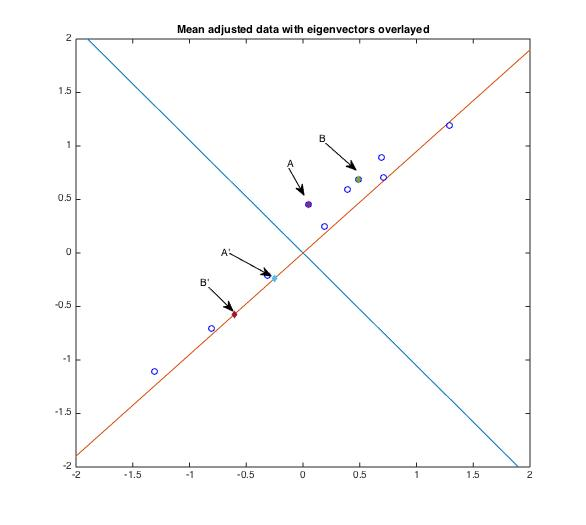
\includegraphics[width=10cm, height=10cm]{4e}
  \end{figure}
  
  \item[f.] 
  $A = (0.05,0.45),B = (0.49,0.69)$
  
 $ A\prime = [-0.7253,-0.6885]*A = -0.3461$
 
$  B\prime = [-0.7253,-0.6885]*B = -0.8304
  $
  %\controlprint{\bigv}
  \\
  \\

\end{enumerate}
\section*{Mini Machine Problem 1 }

\textbf{Answers} 


\begin{enumerate}
\item[1.] Load the data \textbf{carsmall} in Matlab using the following code.
\begin{lstlisting}
load carsmall
X = [MPG,Acceleration,Displacement,Weight,Horsepower];
varNames = {'MPG'; 'Acceleration'; 'Displacement'; 'Weight'; 'Horsepower'};
\end{lstlisting}
\item[2.] (Comet graph is an animated graph. To trace the data points on the screen for the \texttt{Displacement} attribute, we use the following code to visualize the \texttt{Displacement} attribute. Show the \textbf{final comet graph} in the PDF file you will submit by running the following code on Matlab.
\begin{lstlisting}
comet(Displacement)
xlabel('Index of Car')
ylabel('Displacement')
\end{lstlisting}

  \begin{figure}[h]
  \centering
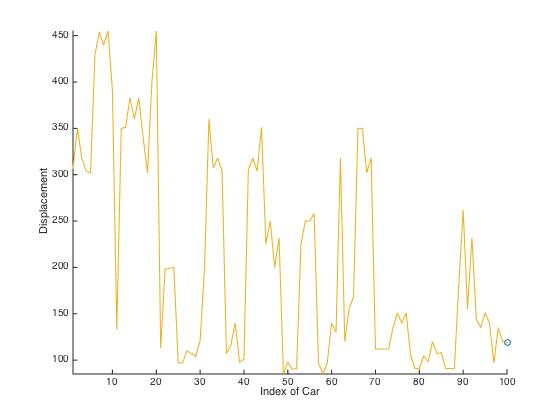
\includegraphics[width=10cm, height=10cm]{mp12}
  \end{figure}
  

\item[3.] (5') Drawing boxlpot is a popular way to visualize a distribution. The two whiskers show the Min observation and the Max observation. The central line shows the median. The edges of the box are the first quantile and the third quantile. 
\begin{itemize}
\item[a.] (1') Run the following code on your Matlab to draw a boxplot for the \texttt{Acceleration} attribute. Show the \textbf{boxplot}  in the PDF file you will submit.
\begin{lstlisting}
boxplot(Acceleration)
ylabel('Acceleration')
\end{lstlisting}
  \begin{figure}[h]
  \centering
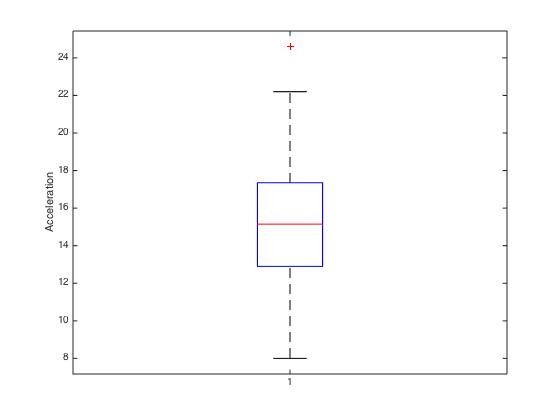
\includegraphics[width=10cm, height=10cm]{mp13a}
  \end{figure}
  

\item[b.] 

\begin{lstlisting}
boxplot(Acceleration,Cylinders)
xlabel('Cylinders')
ylabel('Acceleration')
\end{lstlisting}

  \begin{figure}[H]
  \centering
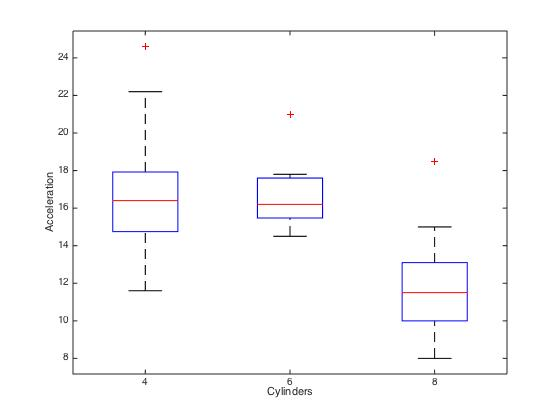
\includegraphics[width=10cm, height=10cm]{mp13b}
  \end{figure}
  

\item[4.] (4') 3-D scatter plots are popularly used to visualize 3 attributes at the same time. 
\begin{itemize}
\item[a.] (2') Run the following code to draw a 3-D scatter plot. Show the \textbf{3-D plot} in the PDF file you will submit. 
\begin{lstlisting}
scatter3(Displacement,Cylinders,Horsepower,'filled','r')
xlabel('Displacement')
ylabel('Cylinders')
zlabel('Horsepower')

\end{lstlisting}
  \begin{figure}[H]
  \centering
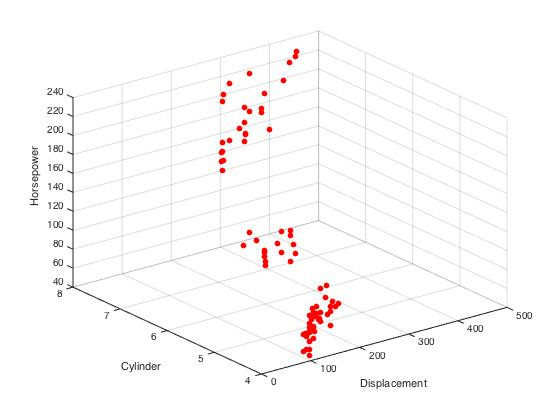
\includegraphics[width=10cm, height=10cm]{mp14}
  \end{figure}
  


\item[b.] 
Horsepower and displacement a pair of positively correlated attributes.
Displacement is the total volume of all the cylindets in an engine. Larger engines tend to produce more power, more turque. 
\end{itemize}

\item[5.] (4') Interactive star plots are used to show the values of attributes for each observation. In each star (observation), the spoke length is proportional to the value of that attribute for that observation.
\begin{itemize}
\item[a.] (2') Run the following code. Show the \textbf{graph} in PDF file you will submit.
\begin{lstlisting}
h = glyphplot(X(1:9,:), 'glyph','star', 'varLabels',varNames,...
'obslabels',Model(1:9,:));
set(h(:,3),'FontSize',8);
\end{lstlisting}

  \begin{figure}[H]
  \centering
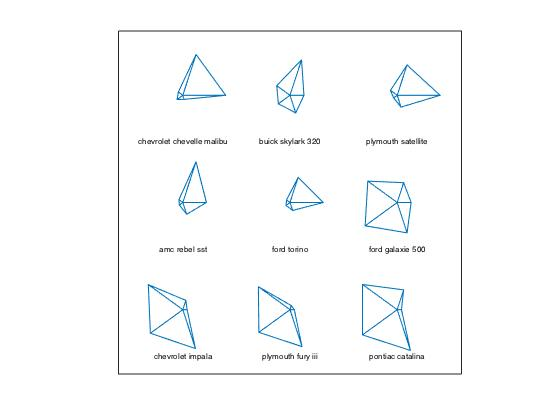
\includegraphics[width=10cm, height=10cm]{mp15}
  \end{figure}
  

\item[b.] 
Observation: Chevrolet chevelle malibu

MPG: 18

Acceleration: 12

Displacement: 307

Weight: 3504

Horsepower: 130

\end{itemize}

\end{enumerate}
\section*{Mini Machine Problem 2 }


\textbf{Answers} 

\begin{enumerate}
\item[1.]  
When $max = 1$, what we do is just to do the exact match. That means each name will match to itself. And the match will always be one. When $max = 0.99$, we are tring to match those names that are similar but not exactly the same. 

 \begin{figure}[H]
  \centering
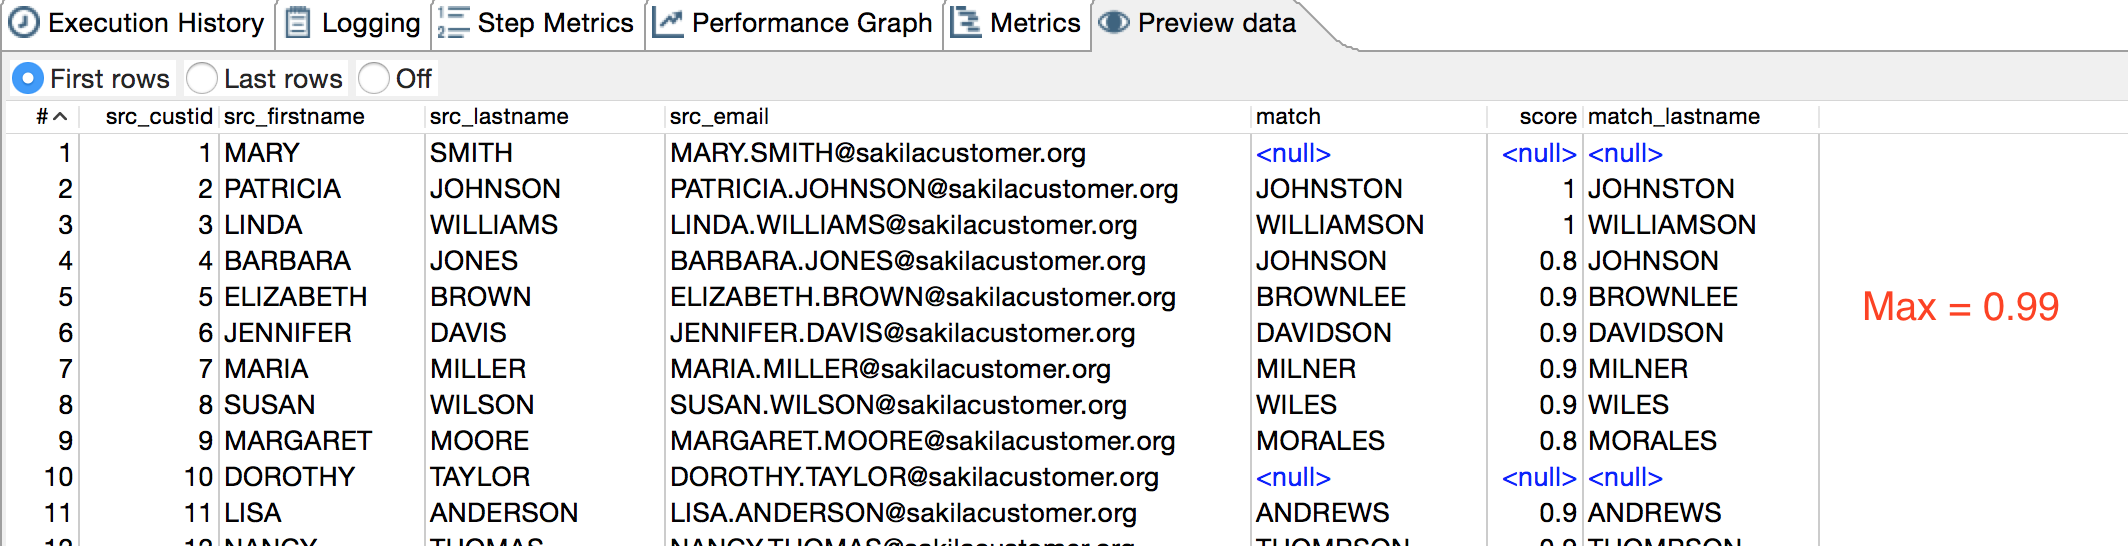
\includegraphics[width=12cm, height=5cm]{max99}
  \end{figure}
  
   \begin{figure}[H]
  \centering
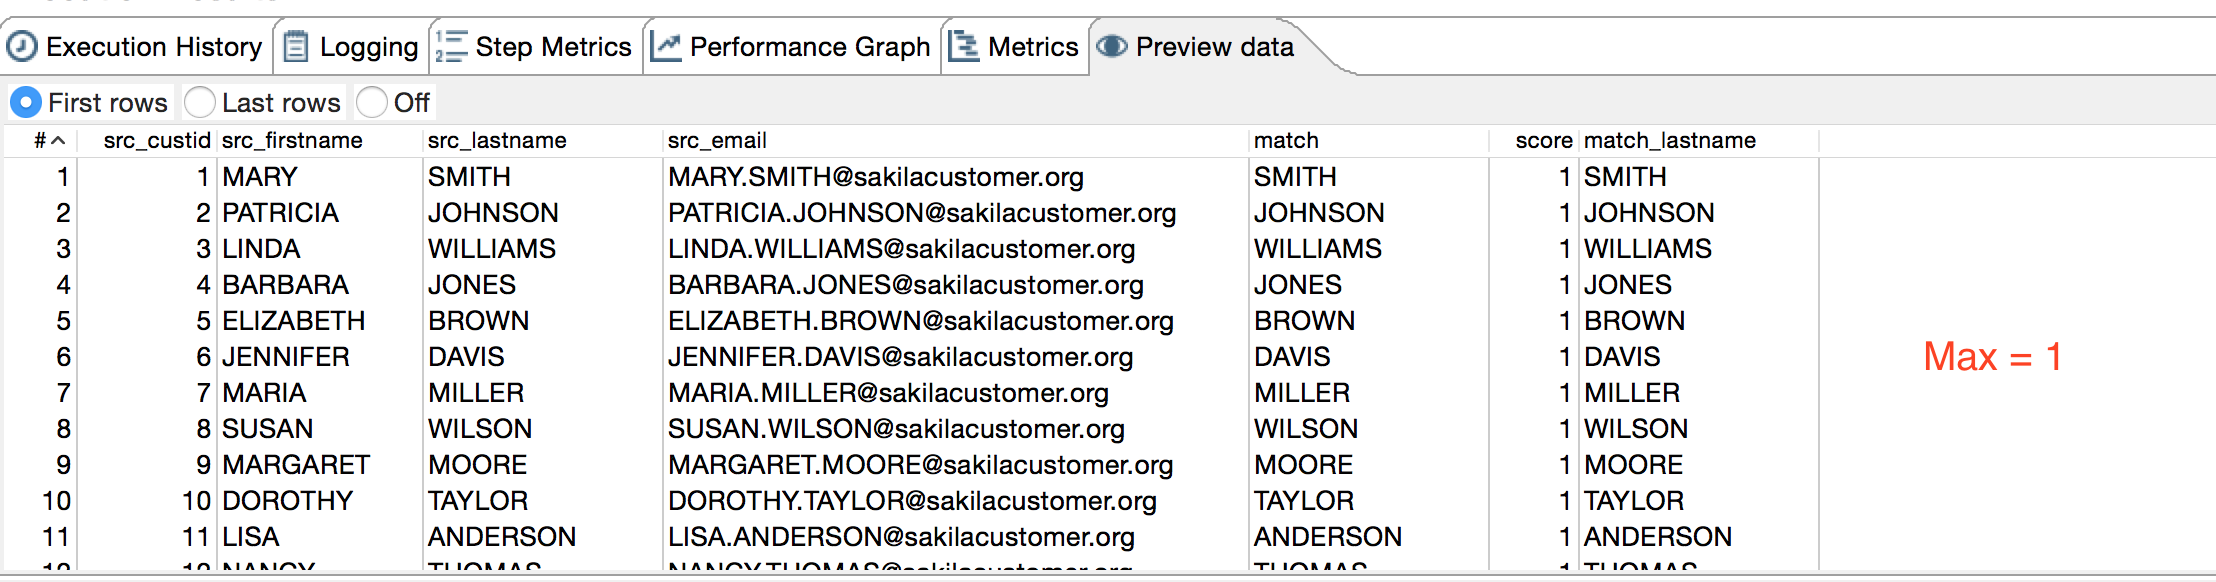
\includegraphics[width=12cm, height=5cm]{max1}
  \end{figure}

\\

\item[2.] 
 \begin{figure}[H]
  \centering
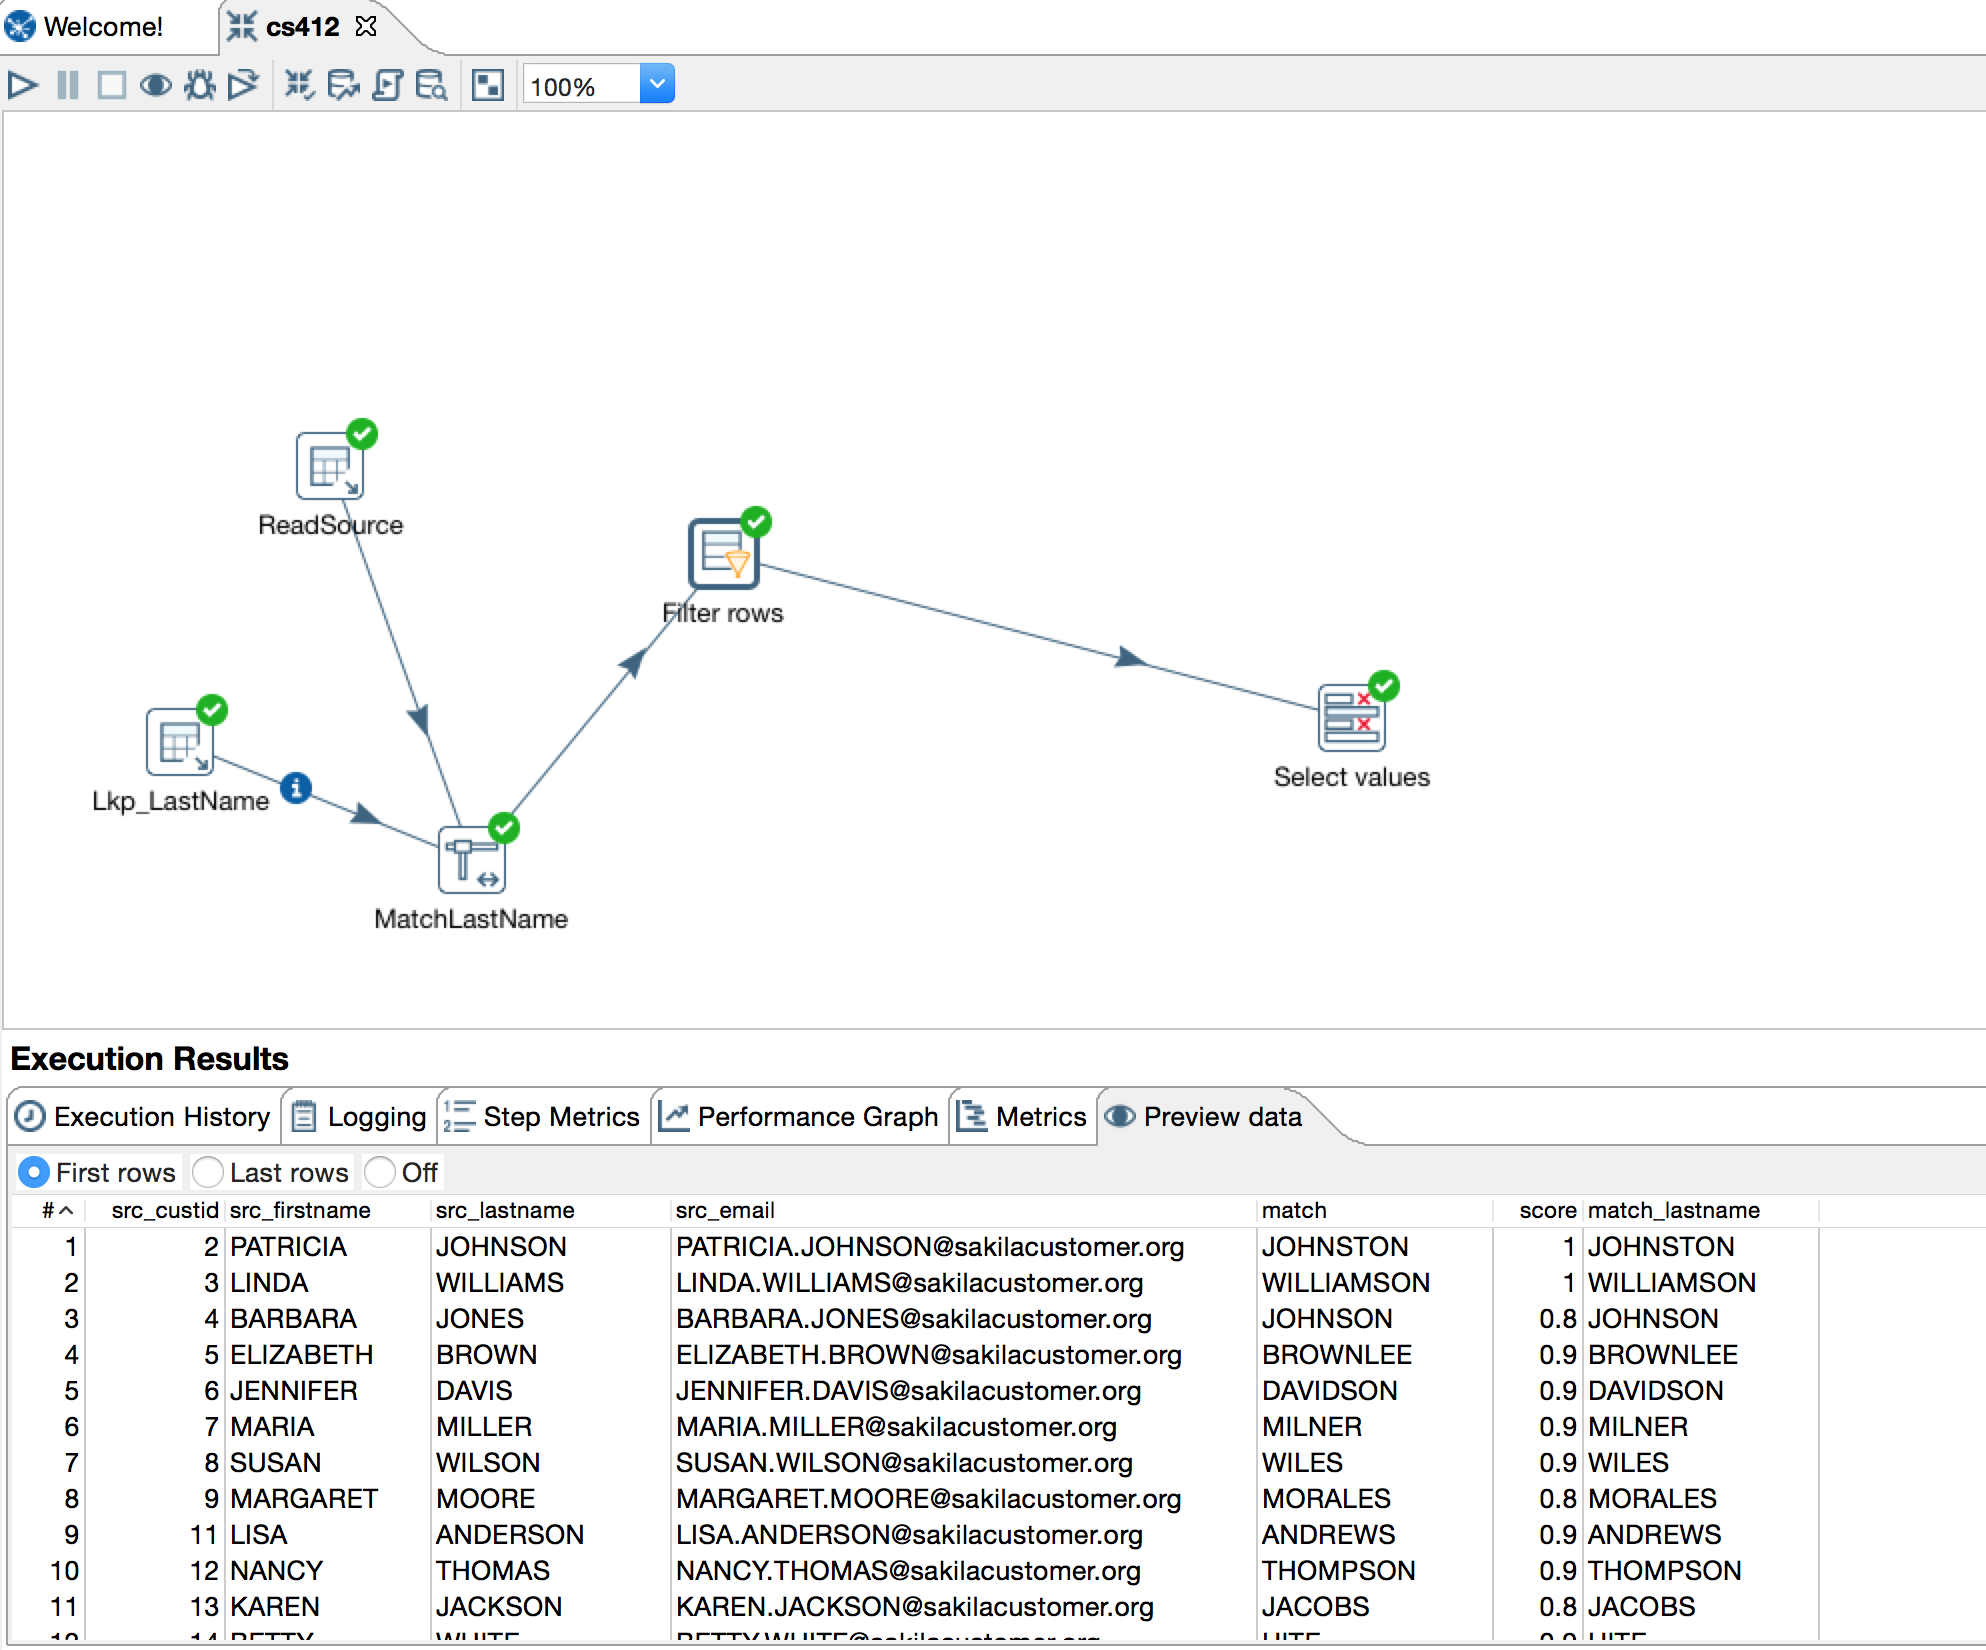
\includegraphics[width=10cm, height=10cm]{mp22}
  \end{figure}
\\

\item[3.] 

 \begin{figure}[H]
  \centering
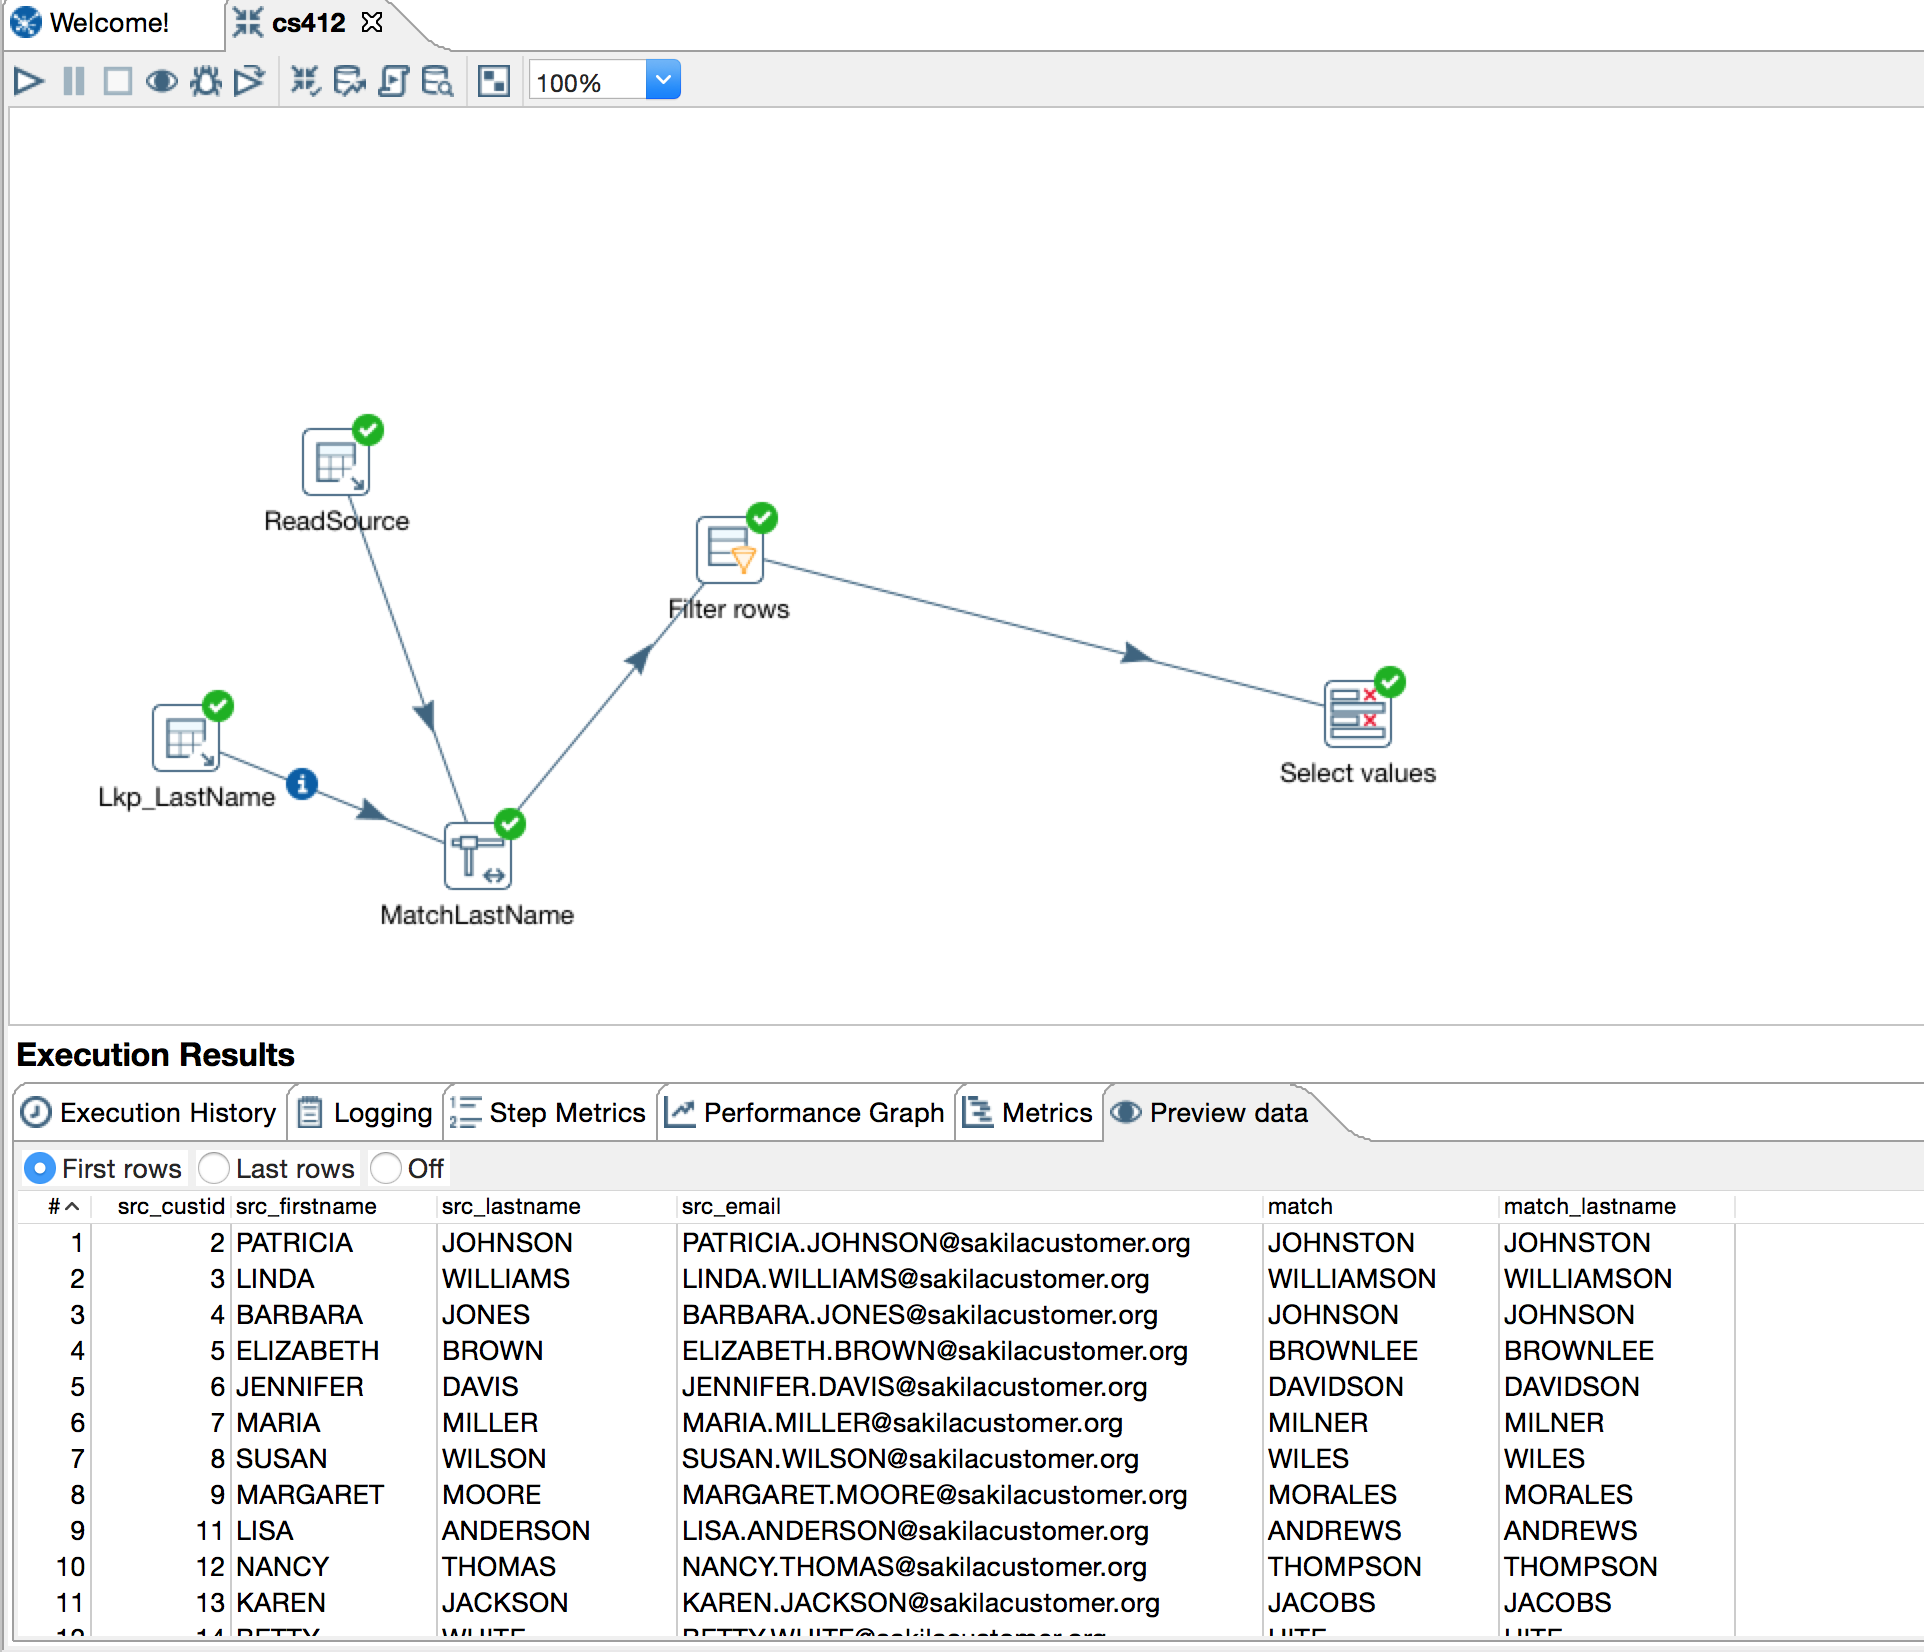
\includegraphics[width=10cm, height=10cm]{mp23}
  \end{figure}
\end{enumerate}

\end{document}